\documentclass[11pt,a4paper]{article}

\usepackage[a4paper,margin=2.15cm]{geometry}
\usepackage[T1]{fontenc}
\usepackage[utf8]{inputenc}
\usepackage{lmodern}
\usepackage{microtype}

\usepackage{graphicx}
\usepackage{xcolor}
\usepackage{booktabs}
\usepackage{tabularx}
\usepackage{longtable}
\usepackage{array}
\usepackage{enumitem}
\usepackage{hyperref}
\usepackage[nameinlink,noabbrev]{cleveref}

\usepackage{tikz}
\usetikzlibrary{arrows.meta,positioning}

\hypersetup{
  colorlinks=true,
  linkcolor=black,
  urlcolor=blue!50!black,
  citecolor=black
}

\setlength{\parindent}{0pt}
\setlength{\parskip}{0.35em}
\setlist[itemize]{noitemsep,topsep=2pt,leftmargin=18pt}
\setlist[enumerate]{noitemsep,topsep=2pt,leftmargin=20pt}
\renewcommand{\arraystretch}{1.12}
\sloppy

\title{\vspace{-1.2cm}\textbf{\Large IEPS --- Assignment 3 Report}\\[0.3em]
\large Retrieval-Augmented Generation over GitHub READMEs\vspace{-0.2cm}}
\author{Tilen Lampret \quad Pika Kri\v{z}nar \quad Grega Rade\v{z}\\Faculty of Computer and Information Science, Ljubljana}
\date{May 2026}

\begin{document}
\maketitle
\small

\begin{abstract}
We built a Retrieval-Augmented Generation (RAG) system on top of the PA2 GitHub README corpus. A query is embedded with MiniLM-L6-v2, matched in PostgreSQL/pgvector (cosine HNSW), reranked with a cross-encoder, and passed as numbered evidence to a local Ollama \texttt{llama3.2:1b} model orchestrated by dspy. The same queries are also answered in an LLM-only mode without retrieval. We evaluated nine queries (six README-grounded, three intentionally out-of-scope) and logged full retrieval traces before generation. When retrieval surfaces on-topic install, training, or evaluation sections, RAG answers are more repository-specific and diagnosable than LLM-only baselines. Failures remain visible: bibliography-dominated retrieval on poor queries, generation that ignores strong evidence (e.g., skipping \texttt{evaluate.py} commands), and hallucinated facts even when the prompt restricts answers to context.
\end{abstract}

\noindent\textbf{Keywords:} retrieval-augmented generation, pgvector, cross-encoder reranking, Ollama, explainability, GitHub README corpus

\section{Introduction}
In PA1 we crawled image-segmentation repositories; in PA2 we extracted README text, segmented it, embedded segments, and demonstrated semantic retrieval. PA3 extends that retrieval stack with a local large language model capable of answering natural-language questions in two different operating modes. The goal of the assignment was not only to generate answers, but also to understand how retrieval affects answer quality, transparency, and trustworthiness.

The implemented system therefore supports the following two modes:

\begin{itemize}
  \item \textbf{With Context (RAG):} retrieve the top relevant segments from the corpus, format them as explicit evidence, and generate an answer conditioned on that evidence.
  \item \textbf{Without Context (LLM-only):} answer the question directly using only the language model without retrieval support.
\end{itemize}

The assignment strongly emphasized explainability. Because of this, our implementation was designed so that all retrieved evidence is visible before generation. The user can inspect the retrieved chunks, see their ranking scores, inspect repository URLs, and determine whether the evidence itself is reliable before trusting the generated answer.

Compared to a standard chatbot pipeline, this architecture makes debugging significantly easier. If the final answer is incorrect, we can separate the problem into two categories:

\begin{enumerate}
  \item retrieval failed and returned poor or irrelevant evidence,
  \item generation failed despite having good evidence available.
\end{enumerate}

This distinction became especially important during evaluation because several answers failed for very different reasons. Some failures happened because the requested information did not exist in the README corpus, while others happened because the small local LLM hallucinated unsupported details even when the retrieval stage returned strong evidence.

This report therefore focuses on three major aspects required by the assignment:

\begin{itemize}
  \item implementation decisions and system architecture,
  \item evaluation of chunking and retrieval quality,
  \item analysis of explainability, hallucination behavior, and retrieval effectiveness.
\end{itemize}

\section{Implementation}

\subsection{Overview}
PA3 extends PA2 with answer generation modules located in \texttt{pa3/rag/}. The retrieval implementation itself was intentionally reused instead of rewritten. The file \texttt{pa3/rag/pa2\_retrieval.py} dynamically imports the retrieval implementation from PA2, ensuring that the same embedding pipeline, vector database structure, and similarity logic are preserved across assignments.

The overall execution flow is implemented inside \texttt{answer\_query()} in \texttt{pipeline.py}. Depending on the selected mode, the pipeline either:

\begin{enumerate}
  \item retrieves evidence chunks,
  \item formats the context,
  \item constructs the final prompt,
  \item sends the request to the local LLM,
  \item stores and prints the results.
\end{enumerate}

In LLM-only mode, the retrieval stage is skipped entirely and the query is directly forwarded to the model with a simplified prompt.

The separation between retrieval and generation proved useful during testing because it allowed us to independently evaluate vector search quality and generation quality. This also simplified experimentation with reranking, top-k retrieval, and prompt formatting.

\subsection{Corpus and document structure (from PA2)}
Documents are GitHub README pages represented as chunk-level evidence. The corpus originates from the PA1 crawl of image-segmentation repositories and was transformed into a searchable retrieval dataset during PA2.

The preprocessing pipeline consisted of three major stages:

\begin{enumerate}
  \item \textbf{Extraction:} HTML pages were cleaned and transformed into structured text. Only the markdown-body subtree was preserved. Heading markers such as \texttt{[H1]}--\texttt{[H6]} were inserted to preserve document hierarchy.

  \item \textbf{Segmentation:} extracted README content was split into semantically meaningful chunks using the \texttt{heading\_structure\_v4} strategy. The segmentation algorithm attempted to preserve section coherence while keeping chunk sizes within the embedding model context budget.

  \item \textbf{Embedding:} each chunk was embedded using MiniLM and stored in PostgreSQL together with metadata such as repository URL, page ID, segment ID, and raw text.
\end{enumerate}

Instead of splitting documents using only fixed token windows, the segmentation strategy tried to preserve README semantics. Installation sections, evaluation commands, training instructions, and dataset descriptions therefore usually remained grouped together. This significantly improved interpretability during retrieval because retrieved chunks often corresponded to meaningful README subsections rather than arbitrary text fragments.

The chosen segmentation approach also improved explainability. When a generated answer referenced a retrieved chunk, the user could directly inspect the original README section and understand where the information came from.

\subsection{Chunking strategy and trade-offs}
The chunking strategy was one of the most important implementation decisions because chunk boundaries directly affect retrieval quality.

Our implementation used heading-aware chunking with approximate token targets between 180 and 320 tokens and a hard cap around 420 tokens. This approach attempted to balance two competing goals:

\begin{itemize}
  \item \textbf{Smaller chunks:} improve retrieval granularity because the retrieved text is usually more focused and specific.
  \item \textbf{Larger chunks:} preserve context continuity and reduce the risk of separating related information.
\end{itemize}

During PA2 segmentation design and inspection of retrieved chunks in PA3, we observed several important trade-offs:

\begin{itemize}
  \item Very small chunks frequently lost important surrounding context. Commands, explanations, and dataset names could become separated across multiple chunks.

  \item Very large chunks often reduced retrieval precision because multiple unrelated README sections became merged together.

  \item Bibliography sections sometimes became highly ranked because they contained many technical keywords even though they were not useful for answering the query.
\end{itemize}

The heading-aware approach performed better than naive fixed-window splitting because README files naturally contain semantically organized sections. Preserving this structure made retrieval results easier to interpret and generally improved answer quality in RAG mode.

\subsection{Embeddings and vector retrieval}

\begin{table}[ht]
\centering
\small
\begin{tabular}{ll}
\toprule
Property & Value \\
\midrule
Model & \texttt{sentence-transformers/all-MiniLM-L6-v2} \\
Parameters & \(\sim 22\) million \\
Dimension & 384 (L2-normalized) \\
Metric / index & Cosine (\texttt{<=>}), HNSW on \texttt{page\_segment.embedding} \\
\bottomrule
\end{tabular}
\caption{Query/document embedding configuration.}
\label{tab:embedding}
\end{table}

The crawled corpus mainly consists of English technical README documentation. Because of this, MiniLM represented a good balance between embedding quality, computational cost, and retrieval speed.

The same embedding model was already used in PA2, which simplified compatibility with the existing pgvector index. Reusing the same embedding space also allowed direct comparison between retrieval-only experiments from PA2 and the RAG pipeline from PA3.

Cosine similarity was used as the primary retrieval metric because embeddings were normalized before storage. The pgvector HNSW index enabled efficient approximate nearest-neighbor retrieval even with tens of thousands of segments.

Although larger embedding models may produce better semantic representations, MiniLM was selected because the assignment emphasized local execution and reproducibility on standard hardware.

\subsection{Reranking}
First-stage vector search retrieves \texttt{candidate\_k=20} segments. These results are then reranked using the cross-encoder model \texttt{cross-encoder/ms-marco-MiniLM-L-6-v2}. After reranking, only the top-5 segments are preserved as final evidence.

The reranking stage was introduced because pure cosine similarity often overemphasized keyword overlap. In technical README corpora this can produce problematic retrieval behavior. Bibliography sections, benchmark tables, or unrelated repositories may contain many overlapping technical terms even when they are not useful for answering the query.

The cross-encoder improves ranking quality because it jointly processes the query and passage instead of comparing only embedding vectors.

We compared vector-only retrieval and reranked retrieval on two representative examples:

\begin{table}[ht]
\centering
\scriptsize
\begin{tabular}{llp{5.8cm}}
\toprule
Query & Mode & Rank-1 segment (URL; \texttt{segment\_id}) \\
\midrule
good\_1 (mIoU eval) & No rerank & FCN-Segmentation-TensorFlow; seg.\ 743653 \\
good\_1 & With rerank & OCNet; seg.\ 755357 (validation mIoU text) \\
poor\_1 (medical 2026) & No rerank & 3D MRI brain tumour (Medical Decathlon); seg.\ 754181 \\
poor\_1 & With rerank & TF-1D-2D pipelines bibliography; seg.\ 741817 \\
\bottomrule
\end{tabular}
\caption{Reranking changes the top hit: for good\_1 it promotes OCNet evaluation content over a generic FCN repository; for poor\_1 both top results remain weak, but reranking still changes ordering behavior.}
\label{tab:rerank-ablation}
\end{table}

The reranking stage noticeably improved several good-query results, especially queries related to training commands, evaluation scripts, or dependency installation. However, reranking could not solve cases where the corpus itself lacked the requested information.

\subsection{Language model and orchestration}

\begin{table}[ht]
\centering
\small
\begin{tabular}{ll}
\toprule
Property & Value \\
\midrule
Runtime & Ollama (local HTTP API, \texttt{localhost:11434}) \\
Model & \texttt{llama3.2:1b} via dspy (\texttt{ollama\_chat/llama3.2:1b}) \\
Parameters & \(\sim 1.3\) billion \\
Preflight & \texttt{ollama\_health.require\_ollama()} before generation \\
\bottomrule
\end{tabular}
\caption{LLM configuration.}
\label{tab:llm}
\end{table}

Generation is handled through Ollama running locally on the machine. The chosen model was \texttt{llama3.2:1b}, a relatively small local language model with approximately 1.3 billion parameters.

The model choice was mainly motivated by:

\begin{itemize}
  \item reproducibility on standard laptops,
  \item low memory requirements,
  \item fast local inference,
  \item compatibility with the assignment requirements.
\end{itemize}

The pipeline uses dspy signatures for structured prompting through \texttt{Predict(SimpleRAG)} and \texttt{Predict(SimpleQA)}. Batch evaluation used signatures by default (\texttt{use\_signature=true}); the CLI also supports \texttt{--plain-prompt} for raw template strings, but we did not run a separate comparison experiment.

Despite these advantages, the small model size also introduced important limitations. The model occasionally ignored explicit prompt instructions, hallucinated unsupported facts, or generated additional information not present in the retrieved evidence.

These limitations became especially visible during poor-query evaluation and represent one of the major observations of the assignment.

\subsection{Prompt construction and context assembly}
RAG and LLM-only templates are defined in \texttt{pa3/rag/prompts.py}.

The RAG prompt explicitly instructs the model to:

\begin{itemize}
  \item answer using only the provided context,
  \item avoid unsupported claims,
  \item cite relevant chunk numbers,
  \item explicitly state when the context is insufficient.
\end{itemize}

The LLM-only prompt is intentionally simpler and only discourages repository-specific hallucinations.

Retrieved chunks are formatted as numbered evidence blocks containing:

\begin{itemize}
  \item retrieval rank,
  \item repository URL,
  \item segment ID,
  \item page ID,
  \item cosine distance or cross-encoder rerank score (depending on mode),
  \item full segment text.
\end{itemize}

This structure makes the retrieval stage transparent and easy to inspect.

Context assembly is handled by \texttt{format\_context()}. The final context is capped at \texttt{max\_context\_chars=7000}. If the context becomes too long, lower-ranked chunks are removed first.

This design choice introduced another trade-off:

\begin{itemize}
  \item larger contexts increase available evidence,
  \item smaller contexts reduce token usage and generation noise.
\end{itemize}

In practice, the 7000-character limit worked reasonably well for README-style technical documentation.

\begin{figure}[ht]
\centering
\resizebox{\textwidth}{!}{%
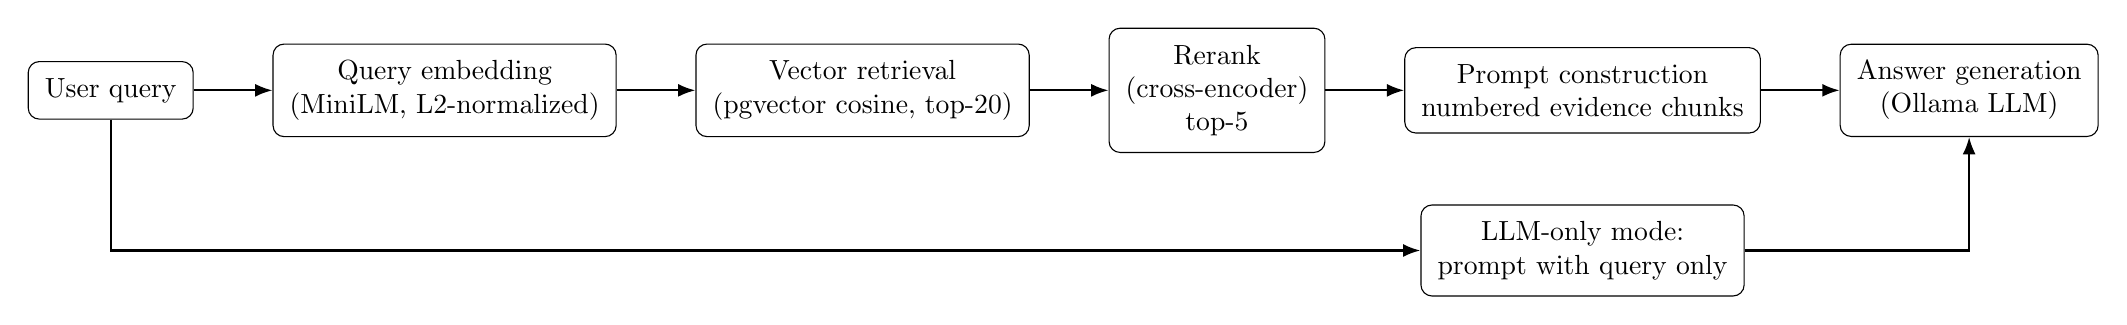
\begin{tikzpicture}[
  node distance=9mm and 10mm,
  box/.style={draw,rounded corners,align=center,inner sep=6pt},
  arrow/.style={-{Latex[length=2.2mm]},thick}
]
\node[box] (q) {User query};
\node[box, right=of q] (emb) {Query embedding\\(MiniLM, L2-normalized)};
\node[box, right=of emb] (vec) {Vector retrieval\\(pgvector cosine, top-20)};
\node[box, right=of vec] (rer) {Rerank\\(cross-encoder)\\top-5};
\node[box, right=of rer] (ctx) {Prompt construction\\numbered evidence chunks};
\node[box, right=of ctx] (gen) {Answer generation\\(Ollama LLM)};

\draw[arrow] (q) -- (emb);
\draw[arrow] (emb) -- (vec);
\draw[arrow] (vec) -- (rer);
\draw[arrow] (rer) -- (ctx);
\draw[arrow] (ctx) -- (gen);

\node[box, below=of ctx] (llm) {LLM-only mode:\\prompt with query only};
\draw[arrow] (q) |- (llm);
\draw[arrow] (llm) -| (gen);
\end{tikzpicture}%
}
\caption{RAG (With Context) and LLM-only (Without Context) pipelines. Hits are logged before generation. The rerank stage is omitted when \texttt{--no-rerank} is set.}
\label{fig:pipeline}
\end{figure}

\textbf{Default configuration:} \texttt{top\_k=5}, \texttt{candidate\_k=20}, reranking enabled, \texttt{max\_context\_chars=7000}.

\subsection{Explainability mechanisms}
One of the most important goals of the project was explainability. Because of this, the system was designed to expose internal retrieval behavior rather than hide it behind the final answer.

The following explainability mechanisms were implemented:

\begin{itemize}
  \item \textbf{CLI tracing:} the command-line interface prints retrieved chunks, scores, URLs, and segment IDs before generation.

  \item \textbf{JSON logging:} complete retrieval traces and generated outputs are stored in \texttt{RunResult} JSON structures.

  \item \textbf{Batch evaluation logging:} \texttt{eval/run\_eval.py} stores retrieval evidence, prompts, context, and answers for all evaluation queries.

  \item \textbf{Failure diagnosis:} retrieval quality and generation quality can be analyzed independently.
\end{itemize}

This architecture proved extremely useful during evaluation because it allowed us to inspect exactly why a generated answer failed.

For example, if the top retrieved chunks are unrelated bibliography entries, then the retrieval stage is responsible. However, if the retrieved chunks clearly contain the correct answer but the model still invents unsupported details, then the problem originates from generation.

Without explicit retrieval logging, these two failure categories would be difficult to distinguish.

\subsection{Libraries and tools}

\begin{table}[ht]
\centering
\small
\begin{tabular}{ll}
\toprule
Component & Library / tool \\
\midrule
Database & PostgreSQL 17 + pgvector \\
DB driver & \texttt{psycopg}, \texttt{pgvector} \\
Bi-encoder / reranker & \texttt{sentence-transformers}, PyTorch \\
LLM orchestration & \texttt{dspy} \\
Local inference & Ollama \\
Evaluation config & PyYAML \\
Data handling & Python standard library + JSON \\
\bottomrule
\end{tabular}
\caption{Main tools used in the implementation.}
\end{table}

Each tool served a different role inside the pipeline. PostgreSQL and pgvector provided efficient vector search capabilities, sentence-transformers handled embedding and reranking models, and Ollama enabled fully local inference without external APIs.

The use of local models also simplified reproducibility because the complete pipeline can run offline once the required models are downloaded.

\section{System evaluation criteria}

\subsection{Data processing evaluation}
The quality of the data processing pipeline was evaluated primarily through retrieval relevance and chunk interpretability.

Because the assignment focused on explainability, it was important that retrieved chunks remain understandable to humans. During evaluation we therefore manually inspected whether retrieved chunks:

\begin{itemize}
  \item preserved semantic coherence,
  \item contained enough context to answer the query,
  \item avoided splitting commands and explanations,
  \item remained small enough for precise retrieval.
\end{itemize}

The heading-aware chunking strategy generally performed well because README files naturally contain structured sections such as:

\begin{itemize}
  \item installation,
  \item training,
  \item evaluation,
  \item dataset preparation,
  \item pretrained model usage.
\end{itemize}

This structure improved retrieval granularity while preserving readability.

However, several weaknesses were also observed:

\begin{itemize}
  \item bibliography-heavy sections sometimes ranked highly,
  \item some merged sections became too broad,
  \item missing README information cannot be recovered by retrieval.
\end{itemize}

The final segmentation strategy represented a compromise between retrieval precision and contextual completeness.

\subsection{Data retrieval evaluation}

\begin{table}[ht]
\centering
\small
\begin{tabular}{ll}
\toprule
Setting & Value \\
\midrule
First-stage retrieval & Cosine similarity, HNSW index \\
Top-\(k\) returned & 5 \\
Candidate pool & 20 \\
Reranker & \texttt{cross-encoder/ms-marco-MiniLM-L-6-v2} \\
\bottomrule
\end{tabular}
\caption{Retrieval settings used during evaluation.}
\label{tab:retrieval}
\end{table}

Retrieval quality was evaluated manually by inspecting whether the returned chunks actually contained information necessary for answering the query.

A retrieved chunk was considered:

\begin{itemize}
  \item \textbf{relevant} if it directly contained commands, metrics, package names, training instructions, or explanations required for the answer,

  \item \textbf{partially relevant} if it belonged to the correct repository but lacked direct answer content,

  \item \textbf{irrelevant} if it consisted mostly of bibliography entries, unrelated repositories, or tangential benchmark discussions.
\end{itemize}

We also analyzed the effect of top-k selection on answer quality.

Using only the top-1 result frequently reduced context coverage too aggressively. On the other hand, very large top-k values introduced noisy evidence and increased the probability of hallucination.

The selected configuration of top-5 reranked chunks represented a practical compromise between evidence diversity and retrieval precision.

The retrieval stage had a direct impact on answer quality:

\begin{itemize}
  \item strong retrieval usually improved specificity and explainability,
  \item weak retrieval often caused vague or hallucinated generation,
  \item missing corpus coverage could not be solved by prompting alone.
\end{itemize}

\subsection{Generation evaluation criteria}
Generation quality was evaluated qualitatively rather than through automatic metrics.

The following aspects were analyzed:

\begin{itemize}
  \item factual consistency with retrieved evidence,
  \item repository specificity,
  \item command correctness,
  \item hallucination frequency,
  \item transparency and explainability.
\end{itemize}

Particular attention was given to cases where the generated answer contained unsupported claims not present in the retrieved evidence.

The assignment specifically emphasized explainability, so we considered an answer more trustworthy when:

\begin{itemize}
  \item retrieved evidence clearly supported the answer,
  \item the answer remained close to the retrieved content,
  \item hallucinated additions were minimized,
  \item the user could verify claims directly from chunks.
\end{itemize}

LLM-only answers were usually less explainable because they lacked explicit supporting evidence.

\subsection{Evaluation protocol}
The evaluation set consisted of nine total queries:

\begin{itemize}
  \item six README-grounded queries expected to succeed,
  \item three intentionally difficult or out-of-scope queries.
\end{itemize}

The original PA2 demo queries were reused and extended with additional repository-specific tasks involving:

\begin{itemize}
  \item dependency installation,
  \item pretrained weights,
  \item custom training.
\end{itemize}

Evaluation was executed using:

\begin{verbatim}
cd pa3/rag
python eval/run_eval.py --output ../output/eval_run.json
\end{verbatim}

Configuration snapshot (2026-05-26):

\begin{itemize}
  \item \texttt{top\_k=5}
  \item \texttt{candidate\_k=20}
  \item reranking enabled
  \item \texttt{llama3.2:1b}
\end{itemize}

Full retrieval traces and generated outputs were stored in \texttt{pa3/output/eval\_run.json} and summarized in \texttt{pa3/output/eval\_run.md}. Reranking impact was analyzed separately using vector-only vs.\ reranked retrieval on the same database snapshot (\Cref{tab:rerank-ablation}).

\section{Results and analysis}

\subsection{Query design}
The evaluation queries were intentionally designed to cover both realistic success cases and realistic failure cases.

\textbf{Good queries (good\_1--good\_6)} focus on information commonly available inside technical README documentation:

\begin{itemize}
  \item evaluation commands,
  \item dataset names,
  \item installation dependencies,
  \item pretrained checkpoints,
  \item training instructions.
\end{itemize}

\textbf{Poor queries (poor\_1--poor\_3)} intentionally require information that static GitHub READMEs cannot reliably provide:

\begin{itemize}
  \item best medical model in 2026,
  \item EU hospital procurement advice,
  \item recent benchmark comparisons.
\end{itemize}

These queries were included because they test whether the system can appropriately fail or acknowledge insufficient evidence.

\subsection{Comparison across nine queries}
\Cref{tab:comparison} summarizes retrieval behavior, generated answers, and overall evaluation.

\begingroup
\scriptsize
\setlength{\tabcolsep}{3pt}
\begin{longtable}{>{\raggedright\arraybackslash}p{1.2cm} >{\raggedright\arraybackslash}p{3.2cm} >{\raggedright\arraybackslash}p{3.4cm} >{\raggedright\arraybackslash}p{3.8cm} >{\raggedright\arraybackslash}p{3.4cm} >{\raggedright\arraybackslash}p{2.1cm}}
\caption{Evaluation comparison: With Context (RAG) vs. Without Context (LLM-only).}\label{tab:comparison}\\
\toprule
ID & Query (short) & Top retrieval & RAG answer (summary) & LLM-only (summary) & Verdict \\
\midrule
\endfirsthead
\toprule
ID & Query (short) & Top retrieval & RAG answer (summary) & LLM-only (summary) & Verdict \\
\midrule
\endhead
\midrule
\multicolumn{6}{r}{(continued on next page)}\\
\endfoot
\bottomrule
\endlastfoot

good\_1 & Evaluate mIoU on validation set & OCNet, DeepLab-v3 (validation commands) & Hyperparameter and OHEM explanation & Generic precision/recall explanation & RAG better \\
good\_2 & Food classification repositories & Food-Categories, Food-Classification-DL & Lists datasets and repositories & Generic food classification statement & RAG better (minor hallucination) \\
good\_3 & SAM inference / checkpoints & SAM-HQ checkpoint usage & Grounded checkpoints; invented \texttt{list\_models()} API & Invented repository URL & Mixed \\
good\_4 & Python dependencies & \texttt{pip install segmentation\_pipeline} & Concrete package names & Generic Python packages & RAG better \\
good\_5 & Download pretrained weights & contrastive-unpaired-translation & Concrete download guidance & Generic model hub answer & RAG better \\
good\_6 & Train on custom dataset & ResNet-50-CBAM, Mask R-CNN & Correct dataset/config workflow & Generic ML checklist & RAG better \\
poor\_1 & Best medical model 2026 & Bibliography-heavy retrieval & Weak fragmented answer & Generic medical AI discussion & Both weak \\
poor\_2 & Hospital EU regulatory purchase & Polyp benchmark text & Irrelevant architecture fragment & Speculative regulatory advice & Both weak \\
poor\_3 & Exact mIoU vs Mask2Former & Benchmark citation blocks & Unsupported metric comparison & Fully hallucinated metrics & Both weak \\
\end{longtable}
\endgroup

\subsection{Good queries: detailed analysis}
For good queries, retrieval generally returned semantically relevant README sections. In these cases, the RAG pipeline consistently produced more repository-specific and more explainable answers than the LLM-only baseline.

The largest improvements appeared in queries involving:

\begin{itemize}
  \item installation instructions,
  \item command-line usage,
  \item pretrained checkpoint downloads,
  \item repository-specific APIs.
\end{itemize}

The retrieval stage helped anchor the model to concrete evidence instead of generic prior knowledge.

\paragraph{good\_1 --- mIoU evaluation query.}
The top retrieved chunks contained validation commands and evaluation scripts from OCNet and DeepLab repositories.

The RAG answer correctly discussed OHEM hyperparameters and validation procedures. However, the model still underused some of the strongest retrieved evidence and failed to directly restate several evaluation commands present in the chunks.

The LLM-only answer instead generated a generic explanation of precision, recall, and sklearn metrics unrelated to the actual repositories.

This example demonstrates that retrieval significantly improved relevance even though generation quality was still imperfect.

\paragraph{good\_2 --- food classification repositories.}
Retrieval correctly identified food-classification repositories and related dataset discussions.

The RAG answer produced repository-specific output and referenced realistic datasets. Food-101 appeared in retrieved chunk \texttt{segment\_id} 754520, but Flickr34, YFCC-100M, and Stanford Food Image Dataset were \textbf{not} present in any top-5 \texttt{segment\_text} (partial hallucination on otherwise good retrieval).

The LLM-only answer remained generic and lacked repository grounding.

This example demonstrates an important observation from the assignment: retrieval can improve relevance while hallucinations still remain possible.

\paragraph{good\_3 --- SAM inference and checkpoints.}
Retrieval returned strong SAM-HQ evidence containing checkpoint download instructions and \texttt{SamPredictor} usage examples.

The RAG answer was mostly grounded in the retrieved evidence but still invented a non-existent \texttt{list\_models()} API.

The LLM-only answer hallucinated an entirely fake repository URL.

This example highlights the difference between partially grounded hallucinations and fully unsupported hallucinations.

\paragraph{good\_4 --- dependency installation.}
The retrieved evidence directly contained dependency installation commands and package lists.

The RAG answer accurately listed relevant packages such as musket-ml, pytorch, torchvision, numpy, and OpenCV.

The LLM-only answer only produced vague references to generic Python dependencies.

This was one of the clearest examples where retrieval strongly improved both answer quality and explainability.

\paragraph{good\_5 --- pretrained weights.}
The retrieval stage returned chunks discussing pretrained checkpoint downloads and repository hosting.

The generated RAG answer remained relatively close to the retrieved evidence and provided useful repository-specific guidance.

The LLM-only answer instead described generic Hugging Face or Keras workflows unrelated to the corpus.

\paragraph{good\_6 --- custom dataset training.}
Retrieved chunks contained dataset folder structures and subclassing examples for custom training.

The RAG answer mirrored the retrieved configuration workflow and remained relatively grounded in the evidence.

The LLM-only answer again defaulted to a generic machine-learning training checklist.

\subsection{Poor queries: detailed analysis}
The intentionally difficult queries revealed several important limitations of the system.

\paragraph{poor\_1 --- best medical model in 2026.}
The retrieval stage returned bibliography-heavy medical segmentation references instead of direct ranking information.

The generated RAG answer became fragmented and incomplete because the evidence itself was insufficient.

The LLM-only answer generated a plausible-sounding medical AI explanation but without reliable support.

This example demonstrates that retrieval quality fundamentally bounds generation quality.

\paragraph{poor\_2 --- EU hospital procurement advice.}
The retrieval stage returned benchmark and architecture descriptions unrelated to procurement or regulation.

The generated answer therefore became meaningless and disconnected from the original question.

The LLM-only answer produced speculative statements about regulations and U-Net architectures despite lacking evidence.

This query demonstrated the limitations of the README-only corpus.

\paragraph{poor\_3 --- exact benchmark comparison.}
Top-ranked chunks were Mask2Former citation blocks without Cityscapes scores. A lower-ranked SeMask segment (\texttt{segment\_id} 745934) contained a 57.52 mIoU value, but nothing in the evidence supported a time-bound comparison to Mask2Former ``last month.''

The RAG answer nevertheless claimed an unsupported SeMask vs.\ Mask2Former comparison. The LLM-only answer hallucinated even larger benchmark values (``\(\sim\)95\% vs.\ \(\sim\)92\%'').

This example demonstrates that prompt instructions alone are insufficient to fully prevent hallucinations in smaller local language models.

\subsection{When retrieval improves answer quality}
Retrieval improved answer quality most strongly when:

\begin{itemize}
  \item the answer existed directly inside README documentation,
  \item retrieved chunks contained commands or configuration examples,
  \item repository-specific terminology was required,
  \item the query closely matched README semantics.
\end{itemize}

The largest improvements were observed in:

\begin{itemize}
  \item installation queries,
  \item dependency queries,
  \item pretrained checkpoint questions,
  \item custom training workflows.
\end{itemize}

In these cases, retrieval significantly increased transparency because users could directly inspect the supporting evidence.

\subsection{When retrieval fails}
Retrieval performed poorly when:

\begin{itemize}
  \item the corpus lacked the requested information,
  \item queries required recent external knowledge,
  \item bibliography sections dominated cosine similarity,
  \item repository README content was too sparse.
\end{itemize}

Even with reranking enabled, the system cannot generate reliable answers if the underlying corpus does not contain relevant evidence.

This became especially visible for regulatory, medical, and time-sensitive benchmark questions.

\subsection{Failure taxonomy and diagnosability}

\begin{table}[ht]
\centering
\small
\begin{tabular}{p{3.2cm}p{7.2cm}p{4.8cm}}
\toprule
Failure type & Symptom & Example queries \\
\midrule
\texttt{irrelevant\_retrieval} & High scores for bibliography/reference sections & poor\_1 \\
\texttt{insufficient\_coverage} & Topic absent from README crawl & poor\_1, poor\_2 \\
\texttt{model\_hallucination} & Claims not present in retrieved chunks & good\_2 (extra datasets), good\_3, poor\_3 \\
\texttt{generative\_without\_evidence} & Plausible but unsupported LLM-only text & good\_2, poor\_1--poor\_3 \\
\bottomrule
\end{tabular}
\caption{Observed failure modes during evaluation.}
\label{tab:failures}
\end{table}

One of the major strengths of the RAG architecture is diagnosability.

Because retrieval evidence is explicitly logged, users can inspect whether the system failure originated from:

\begin{itemize}
  \item retrieval,
  \item corpus coverage,
  \item generation behavior.
\end{itemize}

This transparency is significantly harder to achieve in pure LLM-only systems.

In several evaluation cases, the LLM-only answers appeared more fluent than the RAG answers even though they were less trustworthy. This is an important practical observation because users may incorrectly trust fluent unsupported answers.

The RAG pipeline therefore improves not only answer specificity but also transparency and debuggability.

\section{Limitations and future work}
Several limitations became visible during development and evaluation.

\begin{itemize}
  \item \textbf{README-only corpus:} the dataset does not include GitHub issues, papers, discussions, or external web sources.

  \item \textbf{Small local model:} \texttt{llama3.2:1b} occasionally ignored instructions and hallucinated unsupported details.

  \item \textbf{Reranking limitations:} reranking improves ordering quality but cannot recover missing information.

  \item \textbf{Context truncation:} lower-ranked but useful chunks may be removed when the context becomes too large.

  \item \textbf{No citation verification:} the system does not automatically verify whether generated claims actually appear inside retrieved evidence.

  \item \textbf{Alternative LLMs not used:} the course brief mentions larger or multilingual local models (e.g.\ GaMS, Salamandra); we stayed with \texttt{llama3.2:1b} for speed and reproducibility.
\end{itemize}

Future improvements could include:

\begin{itemize}
  \item larger local LLMs,
  \item explicit hallucination detection,
  \item stricter citation enforcement,
  \item hybrid web retrieval,
  \item automatic confidence estimation,
  \item retrieval score thresholding.
\end{itemize}

A larger evaluation benchmark with human scoring could also provide more rigorous quantitative comparison between RAG and LLM-only modes.

\section{Conclusion}
This project connected the semantic retrieval pipeline from PA2 with a local Retrieval-Augmented Generation architecture capable of transparent evidence-based answering.

The evaluation demonstrated that retrieval substantially improves answer specificity, repository grounding, and explainability for README-based technical questions. RAG answers were generally more informative and easier to verify than LLM-only outputs.

At the same time, the experiments also showed important limitations:

\begin{itemize}
  \item retrieval quality fundamentally bounds generation quality,
  \item missing corpus coverage cannot be solved by prompting,
  \item small local LLMs still hallucinate unsupported details,
  \item fluent answers are not necessarily trustworthy.
\end{itemize}

The most important insight from the assignment was therefore not only how to build a RAG system, but also how retrieval evidence improves transparency and diagnosability.

Even when the generated answer is incorrect, explicit retrieval logging allows users to understand why the system failed. This makes RAG systems significantly easier to debug, evaluate, and trust compared to opaque LLM-only pipelines.

\section*{References}
\begin{itemize}
  \item PA2 pipeline: \texttt{pa2/README.md}
  \item Course RAG demo: \texttt{assignment-2-notebooks/vaje5-RAG\_simple\_demo.ipynb}
  \item PA3 usage and reproduction: \texttt{pa3/README.md}
  \item Evaluation artifacts: \texttt{pa3/output/eval\_run.json}; rerank ablation in \Cref{tab:rerank-ablation} (vector-only vs.\ reranked top-1 on the same DB snapshot)
\end{itemize}

\end{document}